\documentclass[
12pt, % The default document font size, options: 10pt, 11pt, 12pt
%oneside, % Two side (alternating margins) for binding by default, uncomment to switch to one side
onehalfspacing, % Single line spacing, alternatives: onehalfspacing or doublespacing
%draft, % Uncomment to enable draft mode (no pictures, no links, overfull hboxes indicated)
%nolistspacing, % If the document is onehalfspacing or doublespacing, uncomment this to set spacing in lists to single
%liststotoc, % Uncomment to add the list of figures/tables/etc to the table of contents
%toctotoc, % Uncomment to add the main table of contents to the table of contents
%parskip, % Uncomment to add space between paragraphs
%nohyperref, % Uncomment to not load the hyperref package
headsepline, % Uncomment to get a line under the header
%chapterinoneline, % Uncomment to place the chapter title next to the number on one line
%consistentlayout, % Uncomment to change the layout of the declaration, abstract and acknowledgements pages to match the default layout
]{MastersDoctoralThesis} % The class file specifying the document structure

\usepackage[utf8]{inputenc} % Required for inputting international characters
\usepackage[T1]{fontenc} % Output font encoding for international characters
\usepackage{mathpazo} % Use the Palatino font by default

\usepackage[backend=bibtex,style=authoryear,natbib=true]{biblatex} % Use the bibtex backend with the authoryear citation style (which resembles APA)

\addbibresource{example.bib} % The filename of the bibliography

\usepackage[autostyle=true]{csquotes} % Required to generate language-dependent quotes in the bibliography
\usepackage{xcolor}
\usepackage{listings}
%library for networks device
\usepackage{moeptikz}
\usepackage{tikz}
\usepackage{comment}
\usepackage{alltt} 
\usepackage{fancyvrb}
\usepackage{listings} 
\usepackage{xcolor} 
\usepackage{todonotes} 

\lstset{
language=C, 
basicstyle=\small\ttfamily, 
keywordstyle=\color{blue},
keywordstyle=[2]\color{magenta}
keywordstyle=[3]\color{green!50!black} 
stringstyle=\color{red}, 
commentstyle=\color{green!50!black}, % Colore dei commenti 
numbers=left, 
numberstyle=\tiny, % Stile della numerazione
stepnumber=1, % Passo della numerazione 
numbersep=5pt, % Distanza della
tabsize=2, % Dimensione
breaklines=true, % Interruzione automatica delle linee 
morekeywords={include,define}, % Aggiungi le direttive al keyword list
morekeywords=[2]{print},
morekeywords=[3]{return, int, void} 
}

\definecolor{mare}{HTML}{0495ce}

\newcounter{pft}
\usetikzlibrary{decorations.text}
\usetikzlibrary{arrows.meta} 
\usetikzlibrary{positioning, arrows.meta}
\usetikzlibrary{backgrounds,calc,shadings,shapes.arrows,shapes.symbols,shadows}
\usetikzlibrary{matrix, decorations.pathreplacing}
% Definizione del comando per l'evidenziazione del codice inline
\newcommand{\inlinecode}[1]{\colorbox{gray!10}{\texttt{#1}}}
%----------------------------------------------------------------------------------------
%	MARGIN SETTINGS
%----------------------------------------------------------------------------------------

\geometry{
	paper=a4paper, % Change to letterpaper for US letter
	inner=2.5cm, % Inner margin
	outer=3.8cm, % Outer margin
	bindingoffset=.5cm, % Binding offset
	top=1.5cm, % Top margin
	bottom=1.5cm, % Bottom margin
	%showframe, % Uncomment to show how the type block is set on the page
}

%----------------------------------------------------------------------------------------
%	THESIS INFORMATION
%----------------------------------------------------------------------------------------

\thesistitle{Thesis Title} % Your thesis title, this is used in the title and abstract, print it elsewhere with \ttitle
\supervisor{Dr. Paolo \textsc{Santini}} % Your supervisor's name, this is used in the title page, print it elsewhere with \supname
\examiner{} % Your examiner's name, this is not currently used anywhere in the template, print it elsewhere with \examname
\degree{Doctor of Computer Sciences} % Your degree name, this is used in the title page and abstract, print it elsewhere with \degreename
\author{Davide \textsc{De Zuane}} % Your name, this is used in the title page and abstract, print it elsewhere with \authorname
\addresses{} % Your address, this is not currently used anywhere in the template, print it elsewhere with \addressname

\subject{Biological Sciences} % Your subject area, this is not currently used anywhere in the template, print it elsewhere with \subjectname
\keywords{} % Keywords for your thesis, this is not currently used anywhere in the template, print it elsewhere with \keywordnames
\university{\href{http://www.university.com}{Università Politecnica delle Marche}} % Your university's name and URL, this is used in the title page and abstract, print it elsewhere with \univname
\department{\href{http://department.university.com}{Dipartimento di Ingegneria dell'Informazione}} % Your department's name and URL, this is used in the title page and abstract, print it elsewhere with \deptname
\group{\href{http://researchgroup.university.com}{Research Group Name}} % Your research group's name and URL, this is used in the title page, print it elsewhere with \groupname
\faculty{\href{http://faculty.university.com}{Faculty Name}} % Your faculty's name and URL, this is used in the title page and abstract, print it elsewhere with \facname

\AtBeginDocument{
\hypersetup{pdftitle=\ttitle} % Set the PDF's title to your title
\hypersetup{pdfauthor=\authorname} % Set the PDF's author to your name
\hypersetup{pdfkeywords=\keywordnames} % Set the PDF's keywords to your keywords
}

\begin{document}

\frontmatter % Use roman page numbering style (i, ii, iii, iv...) for the pre-content pages

\pagestyle{plain} % Default to the plain heading style until the thesis style is called for the body content

%----------------------------------------------------------------------------------------
%	TITLE PAGE
%----------------------------------------------------------------------------------------

\begin{titlepage}
\begin{center}

\vspace*{.06\textheight}
{\scshape\LARGE \univname\par}\vspace{0.5cm} % University name
\deptname\\[2cm] % Research group name and department name
\textsc{\Large Tesi di Laurea Magistrale}\\[0.5cm] % Thesis type

\HRule \\[0.4cm] % Horizontal line
{\huge \bfseries \ttitle\par}\vspace{0.4cm} % Thesis title
\HRule \\[1cm] % Horizontal line

\begin{figure}[ht!]
	\centering
	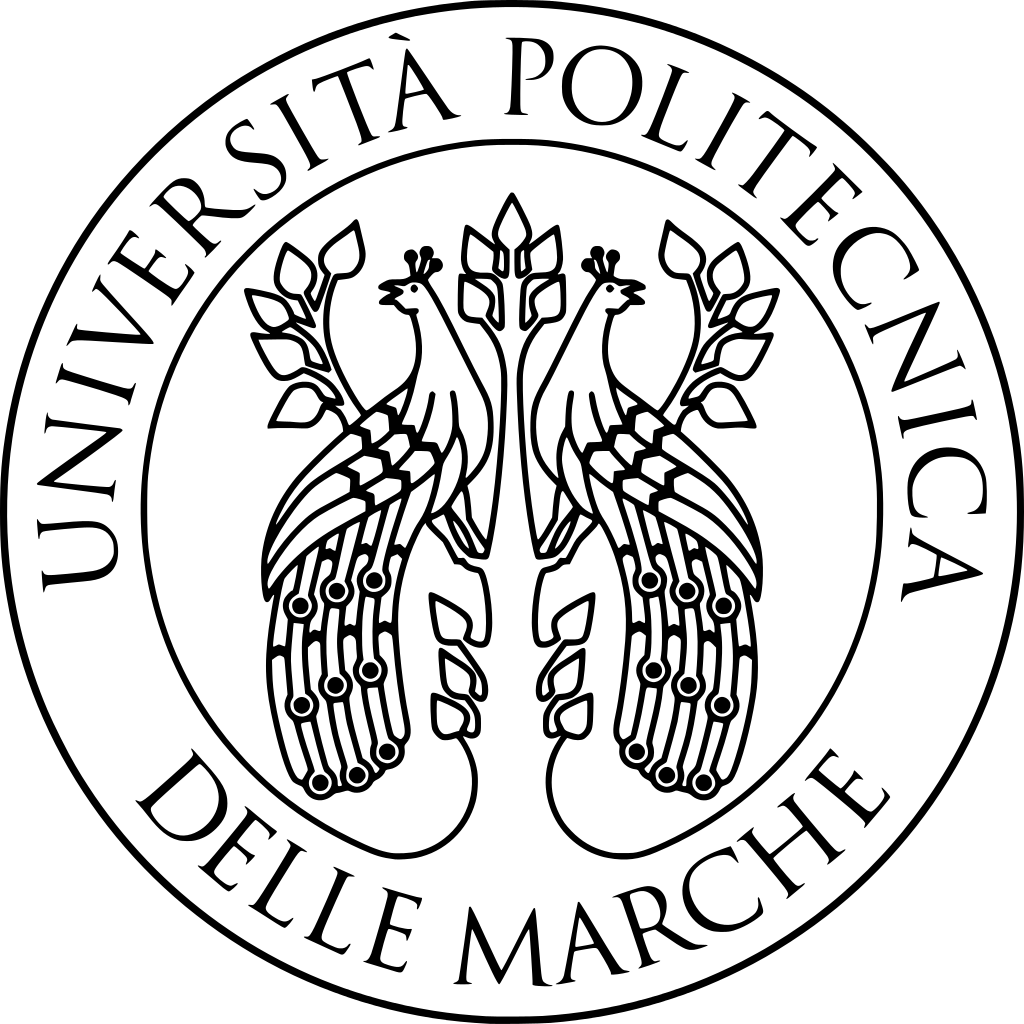
\includegraphics[scale=0.15]{Figures/unvimplogo.png}
\end{figure}
\vspace{1cm}


\begin{minipage}[t]{0.4\textwidth}
\begin{flushleft} \large
\emph{Author:}\\
\href{http://www.johnsmith.com}{\authorname} % Author name - remove the \href bracket to remove the link
\end{flushleft}
\end{minipage}
\begin{minipage}[t]{0.4\textwidth}
\begin{flushright} \large
\emph{Supervisor:} \\
\href{http://www.jamessmith.com}{\supname} % Supervisor name - remove the \href bracket to remove the link  
\end{flushright}
\end{minipage}\\[3cm]
 
\vfill

%\large \textit{A thesis submitted in fulfillment of the requirements\\ for the degree of \degreename}\\[0.3cm] % University requirement text
%\textit{in the}\\[0.4cm]
 
\vfill

{\large \today}\\[4cm] % Date
%\includegraphics{Logo} % University/department logo - uncomment to place it
 
\vfill
\end{center}
\end{titlepage}

%----------------------------------------------------------------------------------------
%	DECLARATION PAGE
%----------------------------------------------------------------------------------------

%\begin{declaration}
%\end{declaration}

%\cleardoublepage

%----------------------------------------------------------------------------------------
%	QUOTATION PAGE
%----------------------------------------------------------------------------------------

\vspace*{0.2\textheight}

\noindent\enquote{\itshape Thanks to my solid academic training, today I can write hundreds of words on virtually any topic without possessing a shred of information, which is how I got a good job in journalism.}\bigbreak

\hfill Dave Barry

%----------------------------------------------------------------------------------------
%	ABSTRACT PAGE
%----------------------------------------------------------------------------------------

\begin{abstract}
\addchaptertocentry{\abstractname} % Add the abstract to the table of contents
The Thesis Abstract is written here (and usually kept to just this page). The page is kept centered vertically so can expand into the blank space above the title too\ldots
\end{abstract}

%----------------------------------------------------------------------------------------
%	ACKNOWLEDGEMENTS
%----------------------------------------------------------------------------------------

\begin{acknowledgements}
\addchaptertocentry{\acknowledgementname} % Add the acknowledgements to the table of contents
The acknowledgments and the people to thank go here, don't forget to include your project advisor\ldots
\end{acknowledgements}

%----------------------------------------------------------------------------------------
%	LIST OF CONTENTS/FIGURES/TABLES PAGES
%----------------------------------------------------------------------------------------

\tableofcontents % Prints the main table of contents

\listoffigures % Prints the list of figures

\listoftables % Prints the list of tables

%----------------------------------------------------------------------------------------
%	ABBREVIATIONS
%----------------------------------------------------------------------------------------

\begin{abbreviations}{ll} % Include a list of abbreviations (a table of two columns)


\textbf{DH} & \textbf{D}iffie \textbf{H}ellman \\
\textbf{KE} & \textbf{K}ey \textbf{E}xchange \\
\textbf{PQ} & \textbf{P}ost \textbf{Q}uantum \\
	
\textbf{IKE} & \textbf{I}nternet \textbf{K}ey \textbf{E}xchange\\
\textbf{KEM} & \textbf{K}ey \textbf{E}ncapsulation \textbf{M}echanism \\
\textbf{PRF} & \textbf{P}seudo \textbf{R}andom \textbf{F}unction \\
\textbf{MTU} & \textbf{M}aximum \textbf{T}ransmission \textbf{U}nit \\
\textbf{ISP} & \textbf{I}nternet \textbf{S}ervice \textbf{P}rovider \\

\end{abbreviations}

%----------------------------------------------------------------------------------------
%	PHYSICAL CONSTANTS/OTHER DEFINITIONS
%----------------------------------------------------------------------------------------

%\begin{constants}{lr@{${}={}$}l} % The list of physical constants is a three column table
% The \SI{}{} command is provided by the siunitx package, see its documentation for instructions on how to use it
%Constant Name & $Symbol$ & $Constant Value$ with units\\
%\end{constants}

%----------------------------------------------------------------------------------------
%	SYMBOLS
%----------------------------------------------------------------------------------------

\begin{symbols}{lll} % Include a list of Symbols (a three column table)

$|$ & concatenazione &  \\
$a$ & distance & \si{\meter} \\
$P$ & power & \si{\watt} (\si{\joule\per\second}) \\
%Symbol & Name & Unit \\

\addlinespace % Gap to separate the Roman symbols from the Greek

$\omega$ & angular frequency & \si{\radian} \\

\end{symbols}

%----------------------------------------------------------------------------------------
%	DEDICATION
%----------------------------------------------------------------------------------------

\dedicatory{For/Dedicated to/To my\ldots} 

%----------------------------------------------------------------------------------------
%	THESIS CONTENT - CHAPTERS
%----------------------------------------------------------------------------------------

\mainmatter % Begin numeric (1,2,3...) page numbering

\pagestyle{thesis} % Return the page headers back to the "thesis" style

% Include the chapters of the thesis as separate files from the Chapters folder
% Uncomment the lines as you write the chapters

% Chapter 1

\chapter{Introduction} 

\label{introduction}  

Introduzione al quantum computer e spiegare il nome, ovvero perchè si basa sui principi fisici.
Confronto con il computer classico utilizzato per calcolare la classe di complessità di un problema

L'attuale crittorafia a chiave pubblica è minacciata da due algoritmi pioneri in questo campo ovvero quello di Grover e Shor
Negli utilimi anni la minaccia del quantum computing, in particolare la loro potenza di calcolo
insieme agli algoritmi di Grover e shor ha 
ribaltato quelle che sono le carte in tavola, dato che consentono di risolvere in tempo
polinomiale i problemi su cui si basano gli schemi crittografici più diffusi 
tra cui il problema del logaritmi discreto alla base di DH e la fattorizzazione di numeri 
primi alla base di RSA.

Questo ha spinto a introdurre nuovi schemi di firma basati su problemi matematici più complessi, 
tra questi abbiamo i lattice-based, hash-based, ecc..
Recentemente tra quelli proposti ne sono stati standardizzati diversi, tra questi abbiamo:
kyber, dilithium, classim mceliece 

\section*{Criticità}

\begin{itemize}
	\item Tradeoff tra aumento della complessità con dimensioni chiave e velocità delle operazioni
	\item Requisiti della rete e in generale delle applicazioni
	\item Implementazioni 
	\item Affidabilità e dunque transizione da uno all'alto.
\end{itemize}


Ora il fatto che questi problemi si siano dimostrati computazionalmente onerosi non li rende 
ottimali anche per l'utilizzo pratico su tutte quelle che sono le infrastrutture di rete esistenti.

Questo perchè per contrastare l'incredibile potenza di calocolo del quantum computer occorre 
rendere il problema più complesso che in generale potrebbe portare e dimensioni delle chiavi molto 
grandi oppure ad operazioni di keygen, codifica e decoddifica molto lonte.

Dunque l'algoritmo dal punto di vista matematico soddisfa quelli che sono i requisiti 
tuttavia non è detta che soddisfi quelli che sono i requisiti che lo rendano adatto ad
essere applicato a contesti reali come quello dlele reti di computer.

Oltre ad un problema computazionale abbiamo anche un problema di fiducia dei cofronti di questi algoritmi, 
ovvero dato che sono stati appena introdotti l'implementazione potrebbe peccare da qualche punto di vista
Inoltre fare una transizione così drastica risulta molto problematico.






Io la metterei si dal punto di vista della ricerca ma anche dal punto di vista implementativo, ovvero 
non basta definire solamente nuovi schemi che dal punto di vista teorico possono essere sicuri 
ma questi devono poi trovare un'utilizzo pratico.

L'utilizzo pratico va in contro a diverse problematiche in particolare ha requisiti più stringenti 
che al momento della definizione matematiche dello schema non vengono presi in considerazione.
Si hanno constraint sia di usabilità che di fiducia nei loro confronti
poichè l'approccio standard è quello di aumentare le dimensioni delle chiavi in modo tale da contrapporti all'aumento di
capacità computazionale del quantum computer

Nel caso reale l'autemto di dimensione ha effetti significativi sulle prestazioni della rete
dato che possono portare a problematiche di frammentazione. E va considerata anche la latenza dovuta alle operazioni 
di cifratura e altre cose



\section*{Contributo Apportato}

L'obiettivo di questo lavoro è andare a vedere quali sono gli effetti di applicare primitive di questo 
tipo nei protocolli maggiormenti diffusi per la sicurezza delle comunicazioni.
In particolare considerando il caso specifico di comunicazioni satellitari, che hanno 
constraint importanti sul numero di pacchetti da scambiare e di conseguenza sulla dimesione di quest'utilimi

Una volta determinati quelli che sono gli effetti, siamo passati a verificare se il protocollo utilizzato 
rispetto alla sua applicazione, fosse quello ideale. 
In particolare dalle conclusioni del benchmarcking siamo arrivati ad una prima implementazione, molto spartana,
di quella che è una versione minimale di IKE.



\section*{Organizazione della Tesi}

Il proseguo della tesi sarà strutturato nel seguente modo:

\begin{itemize}
	\item Capitolo 2:  si danno le fondamenta matematica delle sicurezza nelle comunicazioni 
	sicure e di come queste vengono applicte nelle comunicazioni digitali. In particolare
	prendiamo in esame il caso di IPsec e di un suo protocollo ausiliario utilizzato per negoziarne 
	i parametri di sicurezza.
	\item Capitolo 3: descrizione di quello che è lo scenario applicativo che si prende in considerazione 
	
\end{itemize}

%----------------------------------------------------------------------------------------

% Define some commands to keep the formatting separated from the content 
\newcommand{\keyword}[1]{\textbf{#1}}
\newcommand{\tabhead}[1]{\textbf{#1}}
\newcommand{\code}[1]{\texttt{#1}}
\newcommand{\file}[1]{\texttt{\bfseries#1}}
\newcommand{\option}[1]{\texttt{\itshape#1}}

%----------------------------------------------------------------------------------------
% Chapter Template
\newcommand{\drawkey}[3]{
    \draw[line width=0.07cm, draw=#2] (#1) circle [radius=0.15cm];
    \draw[line width=0.07cm, draw=#2] (#1 -0.15) -- ++(0,-0.4);
    \draw[line width=0.07cm, draw=#2] (#1 -0.35) -- ++(-0.2,0);
    \draw[line width=0.07cm, draw=#2] (#1 -0.51) -- ++(-0.2,0);
    \node[below, text=#2] at (#1 -0.6) {#3}
}

% Definizione del comando per disegnare la parentesi
\newcommand{\drawcurlybrace}[3]{% posizione finale, posizione iniziale, testo sopra
    \draw [decorate,decoration={brace,amplitude=10pt,mirror},xshift=-4pt,yshift=0pt]
    (#1) -- (#2) node [black,midway,xshift=-2cm] {};
}

\chapter{Fondamenti di Comunicazioni Sicure}
\label{Capitolo 2} 

In questo capitolo andiamo a trattare quelle che sono le problematiche riguardanti le comunicazioni sicure.
E' possibile realizzare comunicazioni sicure grazie a quelli che cono i crittosistemi, andiamo a vedere come questi vengono utilizzati nelle reti 
di computer per garantire la sicurezza delle comunicazioni.

\section{Teoria}

Introduciamo quelli che sono gli strumenti fondamentali per la crittografia.

\subsection{Hash Function}

\subsection{Schemi crittografici}
Uno schema di cifratura è un insieme di algoritmi e funzioni che definisce come trasformare un messaggio in chiaro (plaintext) in un messaggio cifrato (ciphertext) e viceversa, al fine di garantire la confidenzialità e la sicurezza delle comunicazioni.
Formalmente possiamo rappresentarlo come una quintupla: 

\begin{center}
    \((\mathcal{P}, \mathcal{C}, \mathcal{K}, E, D)\)
\end{center}

\begin{itemize}
    \item \(\mathcal{P}\): Insieme dei messaggi in chiaro (plaintext).
    \item \(\mathcal{C}\): Insieme dei messaggi cifrati (ciphertext).
    \item \(\mathcal{K}\): Insieme delle chiavi utilizzate per la cifratura e decifratura,\textit{key space}.
    \item \(E: \mathcal{K} \times \mathcal{P} \to \mathcal{C}\): Funzione di cifratura.
    \item \(D: \mathcal{K} \times \mathcal{C} \to \mathcal{P}\): Funzione di decifratura.
\end{itemize}

\noindent
Deve esistere una relazione inversa tra le operazioni di cifratura e decifratura:
\begin{equation}
D(k, E(k, m)) = m \quad \forall m \in \mathcal{P}, \, k \in \mathcal{K}
\end{equation}

\noindent
Questa definizione di schema di cifratura è generale, tuttavia in base alla definizione e all'uso delle chiavi, è possibile distinguere tra schemi di cifratura simmetrica e asimmetrica.

\subsubsection{Simmetrici}

In uno schema simmetrico si utilizza la stessa chiave sia per le operazioni di cifratura che di decifratura. 
Significa che le due parti coinvolte nella comunicazione, ovvero che si vogliono scambiare un messaggio devono possedere la stessa chiave segreta (PSK).

Alcuni esempi di crittosistemi simmetrici sono DES, AES,...


\subsubsection{Asimmetrici}

In uno schema di cifratura asimmetrica, vengono utilizzate due chiavi distinte: una chiave pubblica e una chiave privata.

Lo spazio delle chiavi \(\mathcal{K}\) è costituito da una coppia di chiavi \((k_{\text{pub}}, k_{\text{priv}})\), dove:

\begin{itemize}
    \item \(k_{\text{pub}}\) è la chiave pubblica (usata per cifrare) 
    \item \(k_{\text{priv}}\) è la chiave privata (usata per decifrare)    
\end{itemize}

\noindent
Le due chiavi sono matematicamente legate, ma è computazionalmente difficile ottenere la chiave privata a partire da quella pubblica (questa è la base della sicurezza).
Quindi le due funzioni si riscrivono come:

\begin{equation}
    E: \mathcal{K}_{\text{pub}} \times \mathcal{P} \to \mathcal{C}
\end{equation}
\begin{equation}
    D: \mathcal{K}_{\text{priv}} \times \mathcal{C} \to \mathcal{P}
\end{equation}


\begin{figure}[htbp]
    \centering
    \begin{tikzpicture}[node distance=1.5cm]
        \node (entity1) [draw=green, rectangle] {Alice};
        \drawkey{-0.8, -0.8}{black}{$K_{pri}$};
        \drawkey{-1.6, -0.8}{black}{$K_{pub}$};
        \node (entity2) [draw=blue, rectangle, right=of entity1, xshift=3cm] {Bob};
        \draw (entity1) -- ++(0,-5) coordinate (vertical1);
        \draw (entity2) -- ++(0,-5);
        \draw[-stealth] (entity1) ++(0,-1) -- (entity2 |-,-1) node[midway, above, text=black, font=\footnotesize] {$K_{pub}$};
        \draw[stealth-] (entity2) ++(0,-2) -- (entity1 |-,-2) node[midway, above, text=black, font=\footnotesize] {$E(K_{pub},m)$};
    \end{tikzpicture}
    \label{}
    \caption{}
\end{figure}

Successivamente andremo nel dettaglio di quelli che sono i principali utilizzi dei crittosistemi asimmetrici.


\subsubsection*{Scambio di Chiavi}
\subsubsection*{Cifratura Asimmetrica}
\subsubsection*{Firma Digitale}

Alcuni esempi di quelli classici sono: RSA, Diffie-Hellman,..

\subsection{Confronto}

Vediamo le principali differenze tra i due 

Distribuzione delle chiavi KDC e PKI.

\subsection{Sicurezza}

Il \textbf{security level} è una misura della forza che una primitiva crittografica raggiunge rispetto ad attacchi.
Solitamente viene espresso come un numero di “bit di sicurezza”, dove $n$-bit di sicurezza significa che l'attaccante dovrebbe eseguire $2*n$ operazioni per romperlo.

Per i cifrari simmetrici, il \textit{livello di sicurezza} è pari alla dimensione del key-space. Mentre la sicurezza degli algoritmi asimmetrici si basa su problemi matematici che sono efficienti da calcolare in una direzione, ma inefficienti da invertire da parte dell'attaccante.
Tuttavia, gli attacchi contro gli attuali sistemi a chiave pubblica sono sempre più veloci della ricerca a forza bruta dello spazio delle chiavi.

Il NIST (National Institute of Standards and Technology) ha introdotto livelli di sicurezza per gli algoritmi di cifratura asimmetrica e post-quantistica come parte della sua iniziativa per standardizzare algoritmi che resistano anche ai computer quantistici.
I livelli sono definiti in \textit{Tabella \ref{tab:security-levels}}.

% NIST Security Level Table
\renewcommand{\arraystretch}{1.3} 
\begin{table}[ht]
    \centering
    \begin{tabular}{>{\centering\arraybackslash}m{3cm}p{10cm}}
        \hline
        \textbf{Security Level} & \textbf{Descrizione} \\
        \hline
        \textbf{Livello 1} & Sicurezza equivalente alla cifratura simmetrica con chiavi da 128 bit, come AES-128.\\
        \textbf{Livello 2} & Sicurezza equivalente ad attacchi contro SHA-256, con complessità circa pari a 128 bit. Leggermente più sicuro del livello 1. \\
        \textbf{Livello 3} & Sicurezza equivalente alla cifratura simmetrica con chiavi da 192 bit, come AES-192. \\
        \textbf{Livello 4} & Sicurezza equivalente ad attacchi contro SHA-384. Leggermente più sicuro del Livello 3. \\
        \textbf{Livello 5} & Sicurezza equivalente alla cifratura simmetrica con chiavi da 256 bit, come AES-256. \\
        \hline
    \end{tabular}
    \caption{Security Levels definiti dal NIST}
    \label{tab:security-levels}
\end{table}


\section{Applicazioni}

Le principali applicazioni crittografiche utilizzate oggi in contesti reali includono SSL/TLS, PGP, IPsec e tante altre. 
Tali applicazioni si basano su crittosistemi che combinano algoritmi di cifratura, autenticazione e gestione delle chiavi per garantire la riservatezza e l'integrità dei dati scambiati.


Nel contesto delle comunicazioni digitali, la crittografia gioca un ruolo fondamentale per garantire la sicurezza dei dati scambiati tra entità remote. 
Uno dei principali modelli di riferimento per la trasmissione di dati su Internet è il modello TCP/IP, che suddivide il processo di comunicazione in diversi livelli, ciascuno con funzioni specifiche.


Così come per le comunicaizoni di tutti i giorni, anche per quelle che avvengono attravers Internet vogliamo rispettare quelli che sono i requisiti di
sicurezza informatica ovvero garantire:

\begin{itemize}
    \item Confidenzialità 
    \item Integrità
    \item Autenticazione
\end{itemize}

Le comunicazioni seguono il modello ISO/OSI per questo possiamo applicarla a diversi livelli
Come viene applicata la crittografia nelle comunicazioni, quindi i vari metodi con cui la sicurezza è applicata ai vari livelli dello stack network.
Si parla di comunicazioni sicure ma a livello pratico queste come vengono realizzate, esiste una suitte di protocolli che consente di ottenerle.



\subsection{IPsec}

Facciamo un focus sulla sicurezza a livello IP, quindi introduciamo la suite di protocolli IPsec
Le comunicazioni sicure si costruiscono sopra un concetto fondamentale noto come Security Association (SA). 
Le comunicazioni sono protette attraverso l'utilizzo di tre tecniche crittografiche:

\begin{itemize}
    \item Autenticazione
    \item Integrità
    \item Cifratura
\end{itemize}


La comunicazioni possono rendersi sicure a diversi livelli dello stack network, tuttavia farla a livello IP ha il grande vantaggio di progettere le comunicazioni 
per tutte le applicazioni, senza andarne a modificare ciascuna suingolarmente. 


Il protocollo IKEv2, definito nell'\texttt{RFC 7296}, è un protocollo di rete che è responsabile della negoziazione di chiavi crittografiche e dei parametri di sicurezza tra due dispositivi, solitamente chiamati peer.

\begin{figure}[htbp]
    \centering
    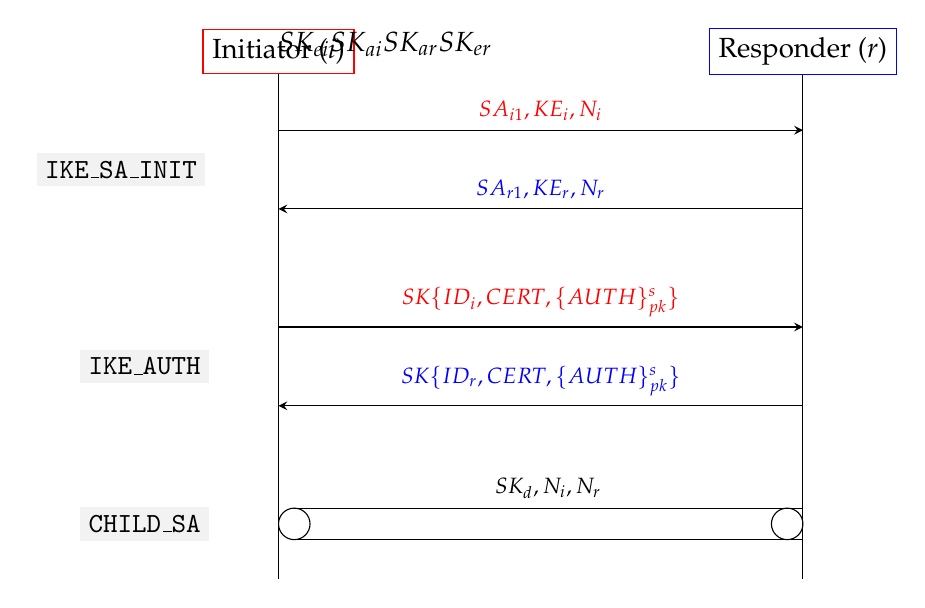
\begin{tikzpicture}[node distance=1.5cm]
        % Initiator and Responder
        \node (entity1) [draw=red, rectangle] {Initiator (\textit{i})};
        \node (entity2) [draw=blue, rectangle, right=of entity1, xshift=3cm] {Responder (\textit{r})};
        \draw (entity1) -- ++(0,-6.7) coordinate (vertical1);
        \draw (entity2) -- ++(0,-6.7);
        % IKE_INIT_SA
        \draw[-stealth] (entity1) ++(0,-1) -- (entity2 |-,-1) node[midway, above, text=red, font=\footnotesize] {$SA_{i1}, KE_i, N_i$};
        \draw[stealth-] (entity1) ++(0,-2) -- (entity2 |-,-2) node[midway, above, text=blue, font=\footnotesize] {$SA_{r1},KE_r,N_r$};
        % IKE_AUTH
        \draw[-stealth] (entity1) ++(0,-3.5) -- (entity2 |-,-3.5) node[midway, above, text=red, font=\footnotesize] {$SK\{ID_i, CERT, \{AUTH\}^s_{pk}\}$};
        \draw[stealth-] (entity1) ++(0,-4.5) -- (entity2 |-,-4.5) node[midway, above, text=blue, font=\footnotesize] {$SK\{ID_r, CERT, \{AUTH\}^s_{pk}\}$};
        % CHILD_SA 
        \node at (-1.7,-6) {\inlinecode{CHILD\_SA}};
        \node at (-2,-1.5) {\inlinecode{IKE\_SA\_INIT}};
        \node at (-1.7,-4) {\inlinecode{IKE\_AUTH}};
        \draw (entity1) ++(0.2,-6) ellipse (0.2cm and 0.2cm);
        \draw [-] (0.2,-6.2) -- (6.65,-6.2);
        \draw [-] (0.2,-5.8) -- (6.65,-5.8) node[midway, above, font=\footnotesize]{$SK_d, N_i, N_r$};
        \draw (entity2) ++(-0.2,-6) ellipse (0.2cm and 0.2cm);
        % Key for encryption and authtenticatoin
        \drawkey{-1, -2.3}{red}{$SK_{ei}$};
        \drawkey{-1.8, -2.3}{red}{$SK_{ai}$};
        \drawkey{8, -2.3}{blue}{$SK_{ar}$};
        \drawkey{8.8, -2.3}{blue}{$SK_{er}$};
        % Group
        \drawcurlybrace{0,-1}{0, -2}{};
        \drawcurlybrace{0,-3.5}{0, -4.5}{};
    \end{tikzpicture}
    \label{fig:ike_exchange}
    \caption{Fasi di Negoziazione del Protocollo IKEv2}
\end{figure}

Lo schema generale di funzionamento del protocollo al termine del quale i due hanno stabilito una SA è riportato in \textit{Fig. \ref{fig:ike_exchange}}.

\subsection{\textbf{IKE\_SA\_INIT}}

Lo scopo di questa prima fase è quello di creare una \textbf{IKE SA}, che consenta di rendere sicure i successivi scambi di dati al fine di realizzare una \textbf{IPsec SA}.
Dunque funge da apripista al fine di stabilire quelli che sono i parametri di sicurezza al fine di avere una comunicazione sicura. Per questo motivo in questo scambio i peer 
si scambiano le seguenti informazioni:

\begin{table}[htbp]
    \centering
    \caption{Tabella dei parametri e delle descrizioni}
    \begin{tabular}{ll}
        \toprule
        \textbf{Parametro} & \textbf{Descrizione} \\
        \midrule
        \textit{SA} & Security Association, vengono negoziati i parametri per la SA\\
        \textit{KE} & Key Exchange, e nel caso classico è l'esponente DH \\
        \textit{N} & Nonce \\
    \bottomrule
    \end{tabular}
\end{table}

\noindent
Al termine di questo scambio i due peer ottengono il \textit{DH Shared Secret} (indicato con $g^{ir}$), il quale insisme ai nonce, consentirà di ottenere 
quelli che sono i parametri di sicurezza della $IKE SA$ al fine di instauare un canale sicuro, per approfondimenti in \href{AppendixA}{appendice}.

% Tabella che riporta le varie funzioni delle chiavi

\subsection{IKE\_AUTH}

Il risultato della fase precedente è un canale sicuro su cui comunicare, in quanto è cifrato e utenticato. Si questo hanno luogo gli scambi per instaurare la IPsec SA.
In questa fase i nodi si autenticano mutuamente:

\begin{table}[htbp]
    \centering
    \caption{Tabella dei parametri e delle descrizioni}
    \begin{tabular}{ll}
        \toprule
        \textbf{Parametro} & \textbf{Descrizione} \\
        \midrule
        \textit{AUTH} & Payload che deve essere firmato affinchè ci sia autenticazione \\
        \textit{CERT} & Si allega il certificato digitale per la chiave pubblica \\
        \textit{CERTQ} & Si fa richiesta al peer di fornire il certificato \\
    \bottomrule
    \end{tabular}
\end{table}

Tutto il contenuto appena descritto è protetto mediante le chiavi segrete di quella direzione. Ciò è indicato mediante la notazione $SK\{...\}$
La modalità di autenticazione può essere: PSK, EAP oppure mediante chiave pubblica.

\subsection{CHILD\_SA}


\section{Problemi}

IKEv2 utilizza come porotocollo a livello trasporto UDP per per inoltrare i propri messaggi. La maggior parte dei messaggi che i peer si scambiano hanno dimensioni relativamente piccole e
quindi che non eccedono l'\textbf{MTU} di un pacchetto IP, tuttavia abbiamo degli scambi che richiedono un trasferimento di dati abbastanza grandi.

Per esempio nel caso di autenticazione tramite pubkey nella fase di \inlinecode{IKE\_AUTH} è necessario trasferire il proprio certificato che in base allo schema di firma utilizzato
può arrivare anche a diversi Kbyte di dimensione. In questi casi si verifica la frammentazione a livello IP.

%Immagine frammentazione

\begin{figure}[htbp]
    \centering
    \begin{tikzpicture}[node distance=2cm,>=Latex]
        % Nodi
        \node (initiator) [client] {Initiator};
        \node (device) [router, right=of initiator] {Device};
        \node (responder) [client, right=of device] {Responder};
        \node (message) [messageclosed, fill=orange!40, minimum size=0.6cm] at (1.9,0.5) {};
        \node (message2) [messageclosed, fill=gray!40, minimum size=0.6cm] at (1.2,0.5) {};
        \node (drop) [messageclosed, fill=gray!40, minimum size=0.6cm, , font=\small, text=red] at (3,1) {};
        \node (message3) [messageclosed, fill=orange!40, minimum size=0.6cm, , font=\small, text=red] at (4.5,0.5) {};

        \draw[-] (initiator.east) -- (device.west);
        \draw[-] (device.east) -- (responder.west);

    \end{tikzpicture}
    \vspace*{1cm}
    \caption{Drop Pacchetti}
    \label{fig:cgnatdrop}
\end{figure}

Diversi test hanno mostrato che nel caso in cui i peer si trovino in presenza di CGNAT potrebbero non istausarsi le SA. Questo è dovuto al fatto che i device degli ISP non
consentono ai frammenti IP di passare attravers di loro, ovvero scartano i pacchetti e di conseguenza bloccano le comunicazioni IKE.
Questo è riportato schematicamente in Fig. \ref{fig:cgnatdrop}.
Questo drop dei pacchetti avviene perchè esistono numerosi vettori di attacco che fanno affidamento sulla frammentazione IP, per questo motivo gli ISP operano un filtro su questa tipologia di pacchetti.
Ance se in teoria uno dei requisiti del CGNAT definito dagli RFC è proprio consentire la frammentazione.

Per risolvere questa problematica e dunque consentire il passaggio dei messaggi attraverso i dispositivi di rete che non consentono il passaggio degli IP fragment attraverso 
di loro nell' RFC 7283 viene introdotta la IKEv2 \textit{Message Fragmentation}. In cui la frammentazione dei messaggi è gestita direttamente da parte di chi implementa IKEv2

\subsection{\inlinecode{IKE\_INTERMEDIATE}}

Per evitare che nel trasferimento di grandi dati ciò avvenga viene introdotto uno scambio aggiuntivo. Questo scambio è introdotto per quei casi in cui la dimensione dei dati
da trasferire ecceda la dimensione massima che causerebbe la frammentazione IP. Questo scambio va fatto dopo la \inlinecode{IKE\_INIT\_SA} e prima della \inlinecode{IKE\_AUTH} in questo
modo è sia autenticato che cifrato tramite le chiavi negoziate dal primo scambio.

\begin{figure}[htbp]
    \centering
    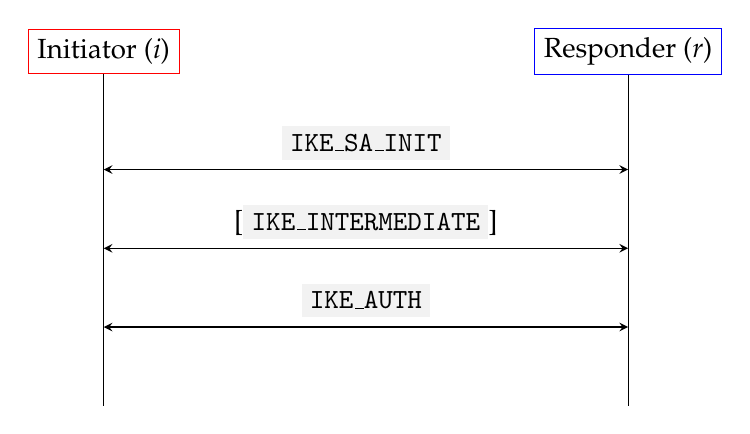
\begin{tikzpicture}[node distance=1.5cm]
        % Initiator and Responder
        \node (entity1) [draw=red, rectangle] {Initiator (\textit{i})};
        \node (entity2) [draw=blue, rectangle, right=of entity1, xshift=3cm] {Responder (\textit{r})};
        \draw (entity1) -- ++(0,-4.5) coordinate (vertical1);
        \draw (entity2) -- ++(0,-4.5);
        % IKE_AUTH
        \draw[stealth-stealth] (entity1) ++(0,-1.5) -- (entity2 |-,-1.5) node[midway, above] {\inlinecode{IKE\_SA\_INIT}};
        \draw[stealth-stealth] (entity1) ++(0,-2.5) -- (entity2 |-,-2.5) node[midway, above] {[\inlinecode{IKE\_INTERMEDIATE}]};
        \draw[stealth-stealth] (entity1) ++(0,-3.5) -- (entity2 |-,-3.5) node[midway, above] {\inlinecode{IKE\_AUTH}};
    \end{tikzpicture}
    \caption{Scambio nuovo}
    \label{fig:ikeintermediate}
\end{figure}

Questo scambio è posizionato qui in quanto nella \inlinecode{IKE\_SA\_INIT} per motivi di sicurezza non è possibile applicare la frammentazione.
Di solito i messaggi sono piccoli abbastanza da non causare la frammentazione IP, tuttavia questo potrebbe cambiare se si utilizzano scambi di chiave QC-resistant; in quanto
hanno chiavi pubbliche larghe e che quindi causerebbero frammentazione IP.

Per questo viene aggiunto questo scambio che viene utilizzato per trasferire grandi quantità di dati.

L'utilizzo principale di questo scambio è quello di trasferire le chiavi pubbliche QC-resistant, tuttavia in generale può essere utilizzzato per trasferire qualsiasi tipologia di dato.
Quindi il principale utilizzo è quello di fare un \textbf{enforcing} delle chiavi negoziate tramite DH al fine di renderle QC-resistant. Infatti se durante questo scambio si scambiano 
altre chiavi allora le coppie $\{SK_{a[i/r]}, SK_{e[i/r]}\}$ vengono aggiornate.

Permette di realizzare Multiple Key Exchange
Gli scambi di chiave aggiuntivi vengono aggiunti alla proposal tramite \inlinecode{PQ\_KEM\_1}



Lo scambio \inlinecode{IKE\_FOLLOWUP\_KE} è introdotto specificatamente per trasferire dati sulla chiavi addizionali da realizzare in una CHILD SA.
In questo caso le chiavi aggiuntive vengono utilizzate per aggiornare il KEYMAT



\begin{itemize}
    \item flag \inlinecode{IKE\_FRAGMENTATION\_SUPPORT}: il peer dice di supportare la frammentazione IKEv2, affinchè venga utilizzata entrambi i peer devono supportarla.
    \item flag \inlinecode{INTERMEDIATE\_EXCHANGE\_SUPPORT}: il peer dice di supportare gli scambi intermedi
\end{itemize}

Una volta terminati gli scambi, per proteggere lo scambio \inlinecode{IKE\_AUTH} e gli scambi successivi vengno utilizzata le ultime chiavi calcolate
Dato che i dati trasferiti in questi scambi aggiuntivi vanno autenticati si aggiungono all'\inlinecode{AUTH} payload che poi andrà 



Il supporto per lo scambio aggiuntivo viene comunicato aggiungendo all'interno
dell \inlinecode{IKE\_SA\_INIT} il flag \inlinecode{IKE\_INT\_SUP} (che sta per
Intermediate Exchange Support).
Se anche il responder lo supporta lo includerà nel messaggio di risposta dello
scambio.




Considerazioni, L'IKE fragmentation viene introdotta a causa del NAT tuttavia nel nostro caso di satelliti non ha senso utilizzarla in quanto non credo che si utilizzi
il NAT soprattutto perchè introduce ritardi dovuti alla traduzione degli indirizzi



\section{Post-Quantum}

Un solo KEM con Kyber L1 usando come suite AES\_GCM has vabene come certificato dilithium L1

Nel KEM quanti cifrano?

Cioè l'initiator manda il certificato e poi il responder cifra  
% Chapter Template

\chapter{Scenario} % Main chapter title

\label{Chapter3} % Change X to a consecutive number; for referencing this chapter elsewhere, use \ref{ChapterX}


%----------------------------------------------------------------------------------------
%	SECTION 1
%----------------------------------------------------------------------------------------

\section{Comunicazioni Satelliari}

Le comunicazioni satellitari sono una fondamenta delle infrastrutture moderne, abilitando una vasta gamma di servizi.
Negli ultimi decenni, con l'aumento della domanda di connettività globale e l'espansione delle reti di telecomunicazioni, i satelliti sono diventati strumenti essenziali per garantire una copertura estesa, specialmente in aree remote dove le infrastrutture terrestri sono limitate o inesistenti.
L'emergere delle costellazioni di satelliti in orbita bassa (LEO - Low Earth Orbit) sta cambiando il paradigma delle comunicazioni satellitari, offrendo vantaggi significativi rispetto ai satelliti geostazionari (GEO). 
%Mentre i satelliti GEO forniscono una copertura stabile, i satelliti LEO consentono Round Time Trip (RTT) notevolmente ridotti e una maggiore flessibilità, rendendoli ideali per applicazioni ad alta velocità come la trasmissione dati in tempo reale e la connettività Internet globale.

Questo cambio di paradigma insieme al quantum computer hanno portato diversi enti, tra cui l'Agenzia Spaziale Europea (ESA), ad affrontare nuove sfide.

\begin{figure}[h!]
    \centering
    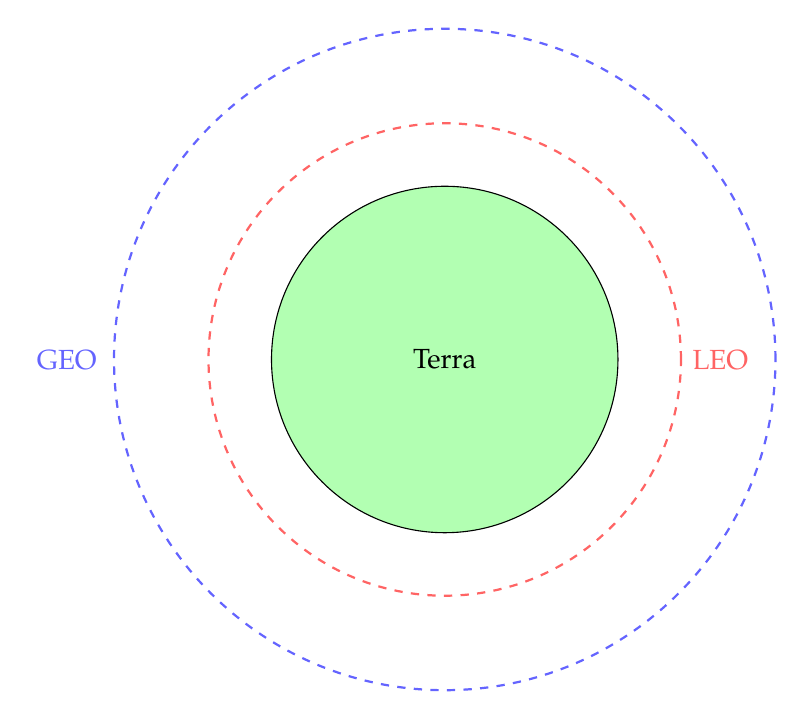
\begin{tikzpicture}
        % Definizione dei colori per le orbite
        \definecolor{leo}{RGB}{255,100,100}
        \definecolor{geo}{RGB}{100,100,255}
        \node at (-4.8, 0) [color=geo]{GEO};
        \node at (3.5, 0) [color=leo]{LEO};
        
        % Cerchio più esterno: l'orbita GEO
        \draw[thick, dashed, geo] (0,0) circle (4.2cm);
        \draw[thick, dashed, leo] (0,0) circle (3cm);
        \filldraw[fill=green!30,] (0,0) circle (2.2cm);
        \node at (0, 0) {Terra};
    \end{tikzpicture}
    \caption{Orbite dei satelliti}
    \label{fig:orbite}
\end{figure}

\subsection{Sfide}

L'ambiente spaziale, caratterizzato da radiazioni intense, temperature estreme e lunghi periodi senza manutenzione, pone sfide significative in termini di progettazione e operatività dell'hardware e del software.
Tra i principali vincoli per l'hardware satellitare troviamo:

\begin{itemize}
    \item \textit{Resistenza alle radiazioni}:
    \item \textit{Basso consumo energetico}: l'energia disponibile per le operazioni computazionali è limitata, quindi si usano processori a basso consumo e ad alta efficienza energetica, sacrificando potenza di calcolo.
    \item \textit{Elaborazione in tempo reale}:
    \item \textit{Compattezza}: lo spazio a disposizione è poco 
\end{itemize}

L'hardware limitato ha un impatto diretto sullo sviluppo del software per i satelliti. 
Rispetto al un contesto terrestre, dove le risorse computazionali sono abbondanti, il software per i satelliti deve essere ottimizzato per funzionare su processori con bassa potenza di calcolo, limitato parallelismo e memoria ridotta. 
Le principali sfide per gli sviluppatori sono:

\begin{itemize}
    \item \textit{Semplicità e ottimizzazione}: gli algoritmi devono essere semplici e ottimizzati per funzionare su hardware con risorse limitate.
    \item \textit{Parallelismo limitato}: non è possibile sfruttare un alto grado di parallelismo computazionale. Le operazioni devono essere eseguite in modo lineare o con limitato parallelismo, aumentando la complessità della progettazione.
    \item \textit{Affidabilità assoluta}: il software deve essere robusto, sicuro e testato ampiamente in modo tale che possibile errori non abbiano conseguenza catastrofiche.
\end{itemize}

Particolare focus va fatto sono le implementazinoni dei protocolli crittografici che si utilizzano per rendere sicure le comunicazioni.
Tuttavia gli algoritmi post quantum, in linea teorica introducono tempi di processamento e dimensioni significative rispetto a quelli classici (carico computazionale elevato).
In questo contesto, diventa essenziale bilanciare sicurezza e prestazioni. Gli algoritmi di crittografia devono essere implementati in modo tale da non compromettere l'efficienza operativa del satellite, riducendo al minimo l'impatto sulle risorse computazionali e di memoria

%-----------------------------------
%	SECTION 2
%-----------------------------------
\section{Come procediamo}

Andiamo a vedere quale è l'impronta in termini comptutazionali delle attuali implementazioni degli algoritmi 
post quantum standardizzati dal NIST, in particolare considerando l'implementazione fornita da open quantum safe (oqs)

E quelle che sono le problematiche che introduce il quantum

In particolare consideriamo la sua integrazione con il protocollo IKE, formita da strongswan dato che siamo in contesto 
satellitare è sensato posizionarsi alla base dello stack.

Andiamo perciò a considerare un'ambiente simulato per confrontare le prestazioni di algoritmi classici rispetto a quelli quantum.
Dato che se la differenza è significativa già in un'ambiente desktop non soggetto a particolari constraint come 
farà ad esserlo nel caso di scenari in cui ci sono numerosi constraint


\section{Benchmarking}
Come abbiamo effettuato il benchmarking
Quindi introdurre tutta la parte di scripting e di automatizazione tramite docker

\section{Tuttavia}

Notiamo che non ci sono enormi differenze in termini di tempi ma tuttavia notiamo una notevole differenza
in termini della dimensione. E in contesto di questo tipo non è auspicabile

Cercando di trovare possibili soluzioni, ci siamo imbattuti su quello che è minimal IKE ovvero
una versione di IKE applicabile in scenari soggetti a constraint di risorse simili a quelli presenti nello spazio.

Riguardo a questo non esistono implementazioni, per questo motivo siamo passati a provare a dare un'implementazione di quest'ultimo
In modo tale che rappresenti un punto di inizio per questo scenario

Di questo trattiamo nel prossimo capitolo

%-----------------------------------
%	SECTION 3
%-----------------------------------



% Chapter Template

\chapter{Hummingbird} % Main chapter title

\label{ChapterX} % Change X to a consecutive number; for referencing this chapter elsewhere, use \ref{ChapterX}

%----------------------------------------------------------------------------------------
%	SECTION 1
%----------------------------------------------------------------------------------------

\section{Progettazione}

\subsection{Requisiti}

Nella parte di progettazione portare quelli che sono i requisiti che deve rispettare l'implementazione
sia funzionali che non
uno tra tutto met

\subsection{Architettura}

Archietettura sia delle directory che a livello dei moduli 
Il C richiede una chiara strutturazione per gestire la complessità del codice in modo efficace

\subsubsection*{Moduli}

Per mantenere la separazione dei compiti

\subsubsection*{Strutture Dati}

%-----------------------------------
%	SECTION 2
%-----------------------------------
\section{Implementazione}

\subsection{Strumenti}

Librerie utilizzate e cose varie, tra queste quelle utilizzate sono:

\begin{itemize}
    \item libcjson: per fare il parsing del file di configurazione scritto in formato json
    \item libcrypto: fornisce le implementazione dei principali schemi crittografici, di hashing e gestione delle chiavi
\end{itemize}

\subsection{Codice}

Il formato dell'header IKE, presente in \textit{Figura \ref{fig:ike-header}}, nel codice \texttt{C}
possiamo tradurlo come una struct


\begin{figure}
    \footnotesize
    \centering
    \begin{Verbatim}[] 
                           1                   2                   3
       0 1 2 3 4 5 6 7 8 9 0 1 2 3 4 5 6 7 8 9 0 1 2 3 4 5 6 7 8 9 0 1 
      +-+-+-+-+-+-+-+-+-+-+-+-+-+-+-+-+-+-+-+-+-+-+-+-+-+-+-+-+-+-+-+-+ 
      |                   Initiator SPI (64 bits)                     |
      +-+-+-+-+-+-+-+-+-+-+-+-+-+-+-+-+-+-+-+-+-+-+-+-+-+-+-+-+-+-+-+-+ 
      |                   Responder SPI (64 bits)                     |
      +-+-+-+-+-+-+-+-+-+-+-+-+-+-+-+-+-+-+-+-+-+-+-+-+-+-+-+-+-+-+-+-+ 
      |  Next Payload |    Version    | Exchange Type |     Flags     |                              
      +-+-+-+-+-+-+-+-+-+-+-+-+-+-+-+-+-+-+-+-+-+-+-+-+-+-+-+-+-+-+-+-+ 
      |                     Message ID (32 bits)                      |
      +-+-+-+-+-+-+-+-+-+-+-+-+-+-+-+-+-+-+-+-+-+-+-+-+-+-+-+-+-+-+-+-+ 
      |                       Length (32bits)                         | 
      +-+-+-+-+-+-+-+-+-+-+-+-+-+-+-+-+-+-+-+-+-+-+-+-+-+-+-+-+-+-+-+-+ 
    \end{Verbatim}
    \caption{Formato IKE Header}
    \label{fig:ike-header}
\end{figure}

\begin{lstlisting} 
    #include <stdio.h> 
    int main() { 
        printf("Hello, World!\n"); 
        return 0; 
    }
\end{lstlisting}
    


Nel parsing della risposta, è stata creata una lookup table. 
Giustificazione dovuta al fatto che la struttura di un pacchetto ike può essere vista come una lista semplicemente puntata
quindi si presta bene ad approcci iterativi. Per questo motivo invece di andare a creare tanti buffer quanti sono i payload si è adottato un approccio diverso

a partire dal buffer del pacchetto si è creata una funzione ricorsiva il cui criterio di stop è quello del next payload nullo (fine della lista), che ad ogni iterazione
si va a "mangiare un pezzo del pacchetto", nel senso che invece che riallocarlo si gioca con i puntatori
una sorta di pacman ma in questo caso il buffer che non consideriamo è ancora esistente, tuttavia questa modalità evita ogni volta di andare a creare e distruggere dei buffer che
sarebbe molto oneroso .

Inoltre è possibile adottare una strategia di buffering pool in cui 

\subsection{Sfide}

%-----------------------------------
%	SECTION 3
%-----------------------------------

\section{Analisi}

%----------------------------------------------------------------------------------------
%	SUBSECTION 2
%----------------------------------------------------------------------------------------

 
%\include{Chapters/Chapter5} 

%----------------------------------------------------------------------------------------
%	THESIS CONTENT - APPENDICES
%----------------------------------------------------------------------------------------

\appendix % Cue to tell LaTeX that the following "chapters" are Appendices

% Include the appendices of the thesis as separate files from the Appendices folder
% Uncomment the lines as you write the Appendices

% Appendix A

\chapter{Tecnico} % Main appendix title

\label{AppendixA} % For referencing this appendix elsewhere, use \ref{AppendixA}


\subsection{Authentication}

L'autenticazione dei peer avviene effettuando il sign (o calcolando il MAC) di un payload che dipende dagli scambi precedenti.
In particolare questo payload è cmposto da un ottetto che viene autenticato in base alla modalità di aunteticazione scelta:

\begin{itemize}
    \item Nel caso di \textit{PubKey} questo viene firmato con la chiave privata del peer e ne viene allegato il certificato della chiave pubblica 
    \item Nel caso di \textit{PSK} l'AUTH payload viene generato a partire dalla chiave condivisa a cui viene aggiunge della unpredicability tramite del padding e una prf
\end{itemize}

\section{Key Derivation}

\subsection{IKE SA}

Le chiavi in una IKE SA vengono derivate a partire dagli attributi dei dirrenti scambi.
In particolare al termine del primo scambio viene calcolato il:

$$SKEYSEED=PRF(N_i|N_r,g^{ir})$$

A partire da questo sidder vengono generati i prametri di sicurezza da utililizzare per la IKE SA, questi sono derivati nel seguente modo:

$$\{SK_{d} | SK_{ai} | SK_{ar} | SK_{ei} | SK_{er} | SK_{pi} | SK_{pr} \} = PRF+(SKEYSEED, N_i|N_r, SPI_i, SPI_r)$$

\begin{table}[htbp]
    \centering
    \begin{tabular}{ll}
        \toprule
        \textbf{Chiave} & \textbf{Descrizione} \\
        \midrule
        $SK_d$ & Utilizzata per generare il keymaterial per le CHILD\_SA \\
        $SK_{a}$ & Chiavi per autenticare gli scambi successivi, una per direzione \\
        $SK_{e}$ & Chiavi per cifrare gli scambi successivi, una per direzione \\
        $SK_{p}$ & Chiavi utilizzata per generare l'AUTH Payload, una per direzione \\
        \bottomrule
    \end{tabular}
    \caption{Chiavi e loro utilizzo}
\end{table}

\subsection{IPsec SA}

Nel caso di una SA questa può essere generata automaticamente dopo l'auth oppure attraverso l'apposito scambio di questo tipo il keymaterial a partire dal quale vengono derivati i parametri di sicurezza è ottenuto nel seguente modo:

$$KEYMAT=prf+(SK_d,  N_i|N_r)$$

Nel caso in cui invece si utilizza lo scambio apposito il key material è ottenuto nel seguente modo


\section{Security Association Payload}

Il Security Association Payload denotato con $SA$ è utlilizzatoper negoziare gli attributi di una Secuiry Association. 
Dunque può contenere molteplici proposte, le quali devono essere ordinate per preferenza, ogni proposal contiene i seguenti algoritmi crittografici:

\begin{itemize}
    \item Encryption Algorithm (ENCR)
    \item Preudorandom Function (PRF)
    \item Integrity Algorithm (INTEG)
    \item Diffie-Hellman Group (KE)
    \item PQ KEM 
\end{itemize}



\newpage

\section{Docker}

Il dockerfile in cui andiamo a containerizzare il servizio è quello in, riferimento al file.
A partire da un'immagine ubuntu andiamo ad installare tutte le utility necessarie, dopodichè 
si scarica il sorgenti di oqs e si compila con i parametri specificati.
Si fa la stessa cosa per strongswan e in fase di confiugrazione si specificano i parametri.
Infine si fa un clean-up del sistema dalle dipendenze necessarie solo per la compilazione.

\begin{lstlisting}[language=Dockerfile]

FROM ubuntu:22.04
RUN DEV_PACKAGES="wget unzip bzip2 make gcc libssl-dev cmake ninja-build"
RUN apt-get update 
    && apt-get install -y iproute2 iputils-ping nano $DEV_PACKAGES 
    && mkdir /liboqs && cd /liboqs 
    && wget linksourcecodeliboqs\$LIBOQS\_VERSION.zip 
    && unzip $LIBOQS_VERSION.zip && cd liboqs-$LIBOQS_VERSION 
    && mkdir build && cd build &&
    && cmake -GNinja -DOQS_USE_OPENSSL=ON \
        -DBUILD_SHARED_LIBS=ON \
        -DCMAKE_INSTALL_PREFIX=/usr \
        -DCMAKE_BUILD_TYPE=Release \
        -DOQS_BUILD_ONLY_LIB=ON .. 
    && ninja && ninja install 
    && cd / && rm -R /liboqs 
    && mkdir /strongswan-build && cd /strongswan-build 
    && wget linksourcecode/strongswan-$VERSION.tar.bz2 
    && tar xfj strongswan-$VERSION.tar.bz2 && cd strongswan-$VERSION 
    && ./configure --prefix=/usr
        --sysconfdir=/etc 
        --disable-ikev1 
        --enable-frodo 
        --enable-oqs
        --enable-silent-rules 
    && make all && make install 
    && cd / && rm -R strongswan-build 
    && ln -s/usr/libexec/ipsec/charon charon 
    && apt-get -y remove \$DEV\_PACKAGES 
    && apt-get -y autoremove && apt-get clean 
    && rm -rf /var/lib/apt/lists/*
EXPOSE 500 4500
ENTRYPOINT ["./charon" ]
\end{lstlisting}

\noindent
Le opzioni \texttt{cap\_add} sono utilizzate per aggiungere capacità specifiche ai container
Docker, consentendo loro di eseguire operazioni che normalmente richiederebbero
privilegi di root. Queelli che servono per il nostr setup sono:

\begin{itemize}
    \item \texttt{NET\_ADMIN} consente al processo all'interno del
    container di eseguire operazioni di amministrazione della rete. 
    Fondamentale per configurare le interfacce di rete e gestire il routing e i
    firewall, operazioni chiave per VPN e IPsec.
    \item \texttt{SYS\_MODULE} consente di caricare e scaricare moduli
    del kernel. Fonda\-mentale per caricare moduli del kernel per supportare 
    funzionalità IPsec che non sono già caricate.
    \item \texttt{SYS\_ADMIN} è una delle capacità più potenti e può
    consentire una vasta gamma di operazioni di amministrazione del sistema.

\end{itemize}

\begin{lstlisting}[style=yaml]
    services: 
        moon: 
            build: ./ 
            container_name: moon 
            cap_add: 
                - NET_ADMIN 
                - SYS_ADMIN 
                - SYS_MODULE 
            volumes: 
                - ./moon:/etc/swanctl 
                - ./strongswan.conf:/etc/strongswan.conf 
        
        carol: 
            build: ./ 
            container_name: carol 
            depends_on: 
                - moon 
            cap_add: 
                - NET_ADMIN 
                - SYS_ADMIN 
                - SYS_MODULE 
            volumes: 
                - ./carol:/etc/swanctl 
                - ./strongswan.conf:/etc/strongswan.conf 
    
\end{lstlisting}

\section{Certificati}

Strongswan mette a disposizione un'utility \texttt{pki} per la gestione della public key infrastrucutre.
Tramite questa utility siamo andati a generare i certificati che serviranno poi per la fase di
mutua autenticazione tra i due peer.
\todo{Vai a vedere su E14 per le dimensioni}
Andiamo a confrontarne la dimensione:
\begin{table}[h]
    \centering
    \begin{tabular}{lcc}
        \toprule
        \textbf{Schema} & \textbf{Chiave private} & \textbf{Certificato} \\
        \midrule
        \texttt{ECDSA} & 227 & 530 \\
        \texttt{falcon512} & 3.0k & 2.4k\\
        \texttt{falcon1024} & 5.6k & 4.5k\\
        \texttt{dilithium2} & 5.3k & 5.4k\\
        \texttt{dilithium3} & 8.2k & 7.6k\\
        \texttt{dilithium5} & 10k & 10k\\
    \end{tabular}
\end{table}
    
Riportare i comandi per generare i certificati e la firma del CA su quelli dei peer
Spiegare che più la catena di certificati diventa lunga più è lungo il processo di autenticazione
e maggiori saranno le dimensioni dei certificati


%\include{Appendices/AppendixB}
%\include{Appendices/AppendixC}

%----------------------------------------------------------------------------------------
%	BIBLIOGRAPHY
%----------------------------------------------------------------------------------------

\printbibliography[heading=bibintoc]

%----------------------------------------------------------------------------------------

\end{document}  
